\documentclass{article}
\usepackage{hyperref}
\usepackage{amsmath}
\usepackage{amssymb}
\usepackage{pgfplots}
\usepackage{float}
\usepackage{todonotes}
\usepackage{tikz}

\renewcommand{\Re}{\mathbb{R}}
\newcommand{\Li}{\mathcal{L}}
\newcommand{\Ex}{\mathbb{E}}
\renewcommand{\Pr}{\mathbb{P}}
\newcommand{\Hy}{\mathcal{H}}

\newcommand\bigO[1]{
    \ensuremath{\mathcal{O}\left(#1\right)}
    }

\newcommand{\sigmoidPlot}{
    
    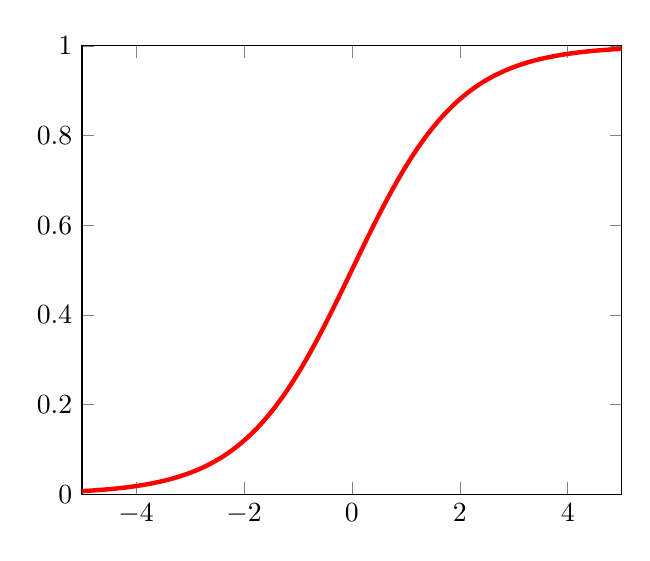
\begin{tikzpicture}
        \begin{axis}[xmin=-5, xmax=5, ymin=0, ymax=1, samples=150]
        \addplot[red, ultra thick] {1/(1+exp(-x))};
        \end{axis}
    \end{tikzpicture}
    
    }

\usetikzlibrary{positioning, calc}
\usetikzlibrary{arrows.meta}

\tikzstyle{circlebox}=[circle,thick,draw=black!75,minimum size=8mm]
\tikzstyle{inputnode}=[circlebox, draw=blue!75]
\tikzstyle{hiddennode}=[circlebox, draw=orange!75]
\tikzstyle{outputnode}=[circlebox, draw=orange!75]
\tikzstyle{simplebox}=[rectangle,thick,draw=black!75,
fill=black!20,minimum size=4mm]
\tikzstyle{textbox}=[rectangle,thick,minimum size=4mm,draw=black!0,
fill=black!0]
\tikzstyle{halfvdistance}=[yshift=-0.7cm]
\tikzstyle{abovebetween}=[xshift=-2.7mm]
\tikzstyle{edgepath} = [-Latex,->,shorten >=1pt,-stealth,semithick, rounded 
corners=5pt]

\def \nodedv {0.735cm}
\def \nodedh {0.65cm}

\tikzset{
    between/.style args={#1 and #2}{
        at = ($(#1)!0.5!(#2)$)
    }
}

\begin{document}
    \section{Subjects}
    \begin{itemize}
        \item Backpropagation
        \item Deep Nets
        \item PCA
        \item Autoencoder
    \end{itemize}
    
    \section{Notes}
    
    \subsection{Neurons and background}
    Neurons consist of a dendritic tree (the input, which branches a lot), the 
    axon (the output, which branches a little bit) and the cell body with 
    nucleus.
    
    Neurons work by having axons connected to dendritic trees, they give a 
    binary ($0$ or $1$) output, after an axon has sent a $1$, it has to 
    recharge.
    
    In order to model this, we've got binary input $x_1,\dots, x_n$ which is 
    sent to the nucleus that sums the inputs together and outputs $1$ if the 
    input exceeds some threshold.
    
    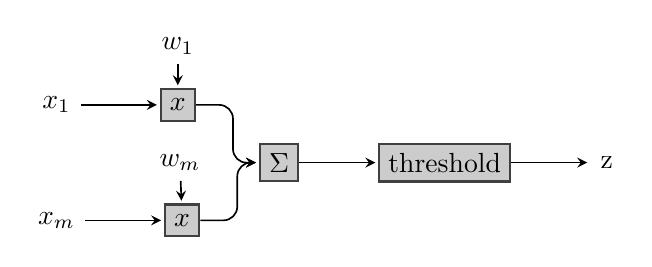
\begin{tikzpicture}
        \node[textbox] (x11) {$x_1$};
        \node[simplebox, right=of x11] (n1) {$x$};
        \node[textbox, above=of n1, halfvdistance] (w1) {$w_1$};
        \path[edgepath]
            (x11) edge node {} (n1)
            (w1) edge node {} (n1);
            
        \node[textbox, below=of x11] (x1m) {$x_m$};
        \node[simplebox, right=of x1m] (nm) {$x$};
        \node[textbox, between=nm and n1] (wm) {$w_m$};
        
        \node[simplebox, right=of n1, between=nm and n1] (sigma1) {$\Sigma$};
        \node[simplebox, right=of sigma1] (threshold1) {threshold};
        \node[textbox, right=of threshold1] (z) {z};
        
        \draw[edgepath]
            (x1m) edge node {} (nm)
            (wm) edge node {} (nm)
            (sigma1) edge node {} (threshold1)
            (threshold1) edge node {} (z);
        \draw[edgepath]
            (n1) -| ++(0.7cm,-\nodedv) -- (sigma1);
        \draw[edgepath]
            (nm) -| ++(0.7cm,\nodedv) -- (sigma1);
    \end{tikzpicture}
    
    This models the following properties:
    \begin{itemize}
        \item All or non
        \item Cumulative influence
        \item Synaptic weight
    \end{itemize}
    But there are more properties that we might like to model, like:
    \begin{itemize}
        \item Refractory period, recovery time of each neuron.
        \item Axonal bifurcation, each pulse will either go down one branch of 
        the axon or the other.
        \item Time patterns, we don't know if the timing of when impulses hit 
        neurons matters.
    \end{itemize}
    So we actually don't know if what we are modelling is the essence of how 
    neurons work or not. But we will start with the simple model.
    
    If we look at what a neural net actually is, then it's a vector of input 
    that goes through a ``box'' which uses some weights and threshold and then 
    outputs some vector $z$. Formally: $z = f(x,w,t)$. So the neural network is 
    just the function $f$, when we train the neural net, all we need to do is 
    change the weights and threshold. We can also think of the neural net as a 
    ``function approximator''.
    
    So, how do we measure the performance of the neural network? If we say the 
    desired result of the neural net $d$ is the function $g$ on the input 
    $x$, $d=g(x)$, then it would be natural to define the performance as: 
    $P=\|d-z\|$, this turns out to be mathematically inconvenient so instead we 
    will use the performance indicator: $P=\|d-z\|^2$.
    
    What we want to do, is of course to maximize the performance. We can do 
    this using gradient descent, for example for the weights $w_1$ and $w_2$:
    \begin{equation*}
        \Delta w= \eta \left(\frac{\partial P}{\partial w_1}i+\frac{\partial 
        P}{\partial w_2}j\right)
    \end{equation*}
    Unfortunately, the function is not linear, and thus gradient descent 
    doesn't really work. This was an issue for a long time untill Paul Werbos 
    figure it out.
    
    First of all, those thresholds are annoying as they are just extra baggage, 
    so we would like to reduce $z$ to be a function of just the inputs and 
    weights:
    \begin{equation*}
        z=f(x,w)
    \end{equation*}
    So what he proposed instead, was adding the bias input to each neuron $w_0$ 
    which is always set to $1$.
    
    
    \begin{tikzpicture}
    \node[textbox, right=of n1, abovebetween] (w0) {$w_0$};
    \node[textbox, right=of w0, yshift=0.5cm, xshift=-0.5cm] (b1) {$1$};
    
    \node[textbox] (x11) {$x_1$};
    \node[simplebox, right=of x11] (n1) {$x$};
    \node[textbox, above=of n1, halfvdistance] (w1) {$w_1$};
    \path[edgepath]
    (x11) edge node {} (n1)
    (w1) edge node {} (n1);
    
    \node[textbox, below=of x11] (x1m) {$x_m$};
    \node[simplebox, right=of x1m] (nm) {$x$};
    \node[textbox, between=nm and n1] (wm) {$w_m$};
    
    \node[simplebox, right=of n1, between=nm and n1] (sigma1) 
    {$\Sigma$};
    \node[simplebox, right=of sigma1] (threshold1) {threshold};
    \node[textbox, right=of threshold1] (z) {z};
    
    \draw[edgepath]
    (x1m) edge node {} (nm)
    (wm) edge node {} (nm)
    (sigma1) edge node {} (threshold1)
    (threshold1) edge node {} (z)
    (b1) edge node {} (w0);
    \draw[edgepath]
        (n1) -| ++(\nodedh,-\nodedv) -- (sigma1);
    \draw[edgepath]
        (nm) -| ++(\nodedh,\nodedv) -- (sigma1);
    \draw[edgepath]
        (w0) -| ++(-\nodedh,-\nodedv) -- (sigma1);
    \end{tikzpicture}
    And then we let $w_0=\text{threshold}$, then the threshold is effectively 
    $1$.\todo{revisit}
    
    Step two, is to smooth the threshold function, which we could do by 
    applying the sigmoid function $\sigma(\alpha)=\frac{1}{1+e^{-\alpha}}$. 
    Then it will be $1$ if $\alpha$ is very big, and $0$ if $\alpha$ is very 
    small.
    \sigmoidPlot
    The generalized term ``activation function'' $\phi$ is in this case 
    $\sigma$, our 
    function is linear and we can take the partial derivatives to the 
    function. Now, suppose we have a very simple neural network:
    
    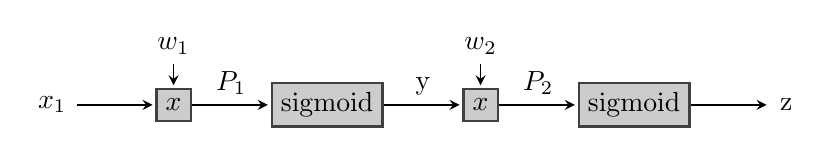
\begin{tikzpicture}
    \node[textbox] (x11) {$x_1$};
    \node[simplebox, right=of x11] (n1) {$x$};
    \node[textbox, above=of n1, halfvdistance] (w1) {$w_1$};
    \node[simplebox, right=of n1] (sigmoid1) {sigmoid};
    
    \path[edgepath]
        (x11) edge node {} (n1)
        (w1) edge node {} (n1)
        (n1) edge node[above] {$P_1$} (sigmoid1);
        
        
    \node[simplebox, right=of sigmoid1] (n2) {$x$};
    \node[textbox, above=of n2, halfvdistance] (w2) {$w_2$};
    \node[simplebox, right=of n2] (sigmoid2) {sigmoid};
    
    \path[edgepath]
        (sigmoid1) edge node[above] {y} (n2)
        (w2) edge node {} (n2)
        (n2) edge node[above] {$P_2$} (sigmoid2);
        
    \node[textbox, right=of sigmoid2] (z) {z};
    
    \path[edgepath]
        (sigmoid2) edge node {} (z);
    \end{tikzpicture}
    
    Now we want to re-write the partial derivative using the chain rule:
    \begin{equation*}
        \frac{\partial P}{\partial w_2} = \frac{\partial P}{\partial z} 
        \frac{\partial z}{\partial w_2} = \frac{\partial P}{\partial z} 
        \frac{\partial z}{\partial p_2} \frac{\partial p_2}{\partial w_2} 
    \end{equation*}
    We can do the same thing for $w_2$:
    \begin{equation*}
        \frac{\partial P}{\partial w_1} = \frac{\partial P}{\partial z} 
        \frac{\partial z}{\partial p_2} \frac{\partial p_2}{\partial y} 
        \frac{\partial y}{\partial p_1} \frac{\partial p_1}{\partial w_1} 
    \end{equation*}
    We can rewrite these two products as:
    \begin{align*}
        \frac{\partial P}{\partial w_2}&= \frac{\partial p_2}{\partial w_2} 
        \frac{\partial z}{\partial p_2} \frac{\partial P}{\partial z}\\
        \frac{\partial P}{\partial w_1}&=\frac{\partial p_1}{\partial w_1} 
        \frac{\partial y}{\partial p_1} \frac{\partial p_2}{\partial y} 
        \frac{\partial z}{\partial p_2} \frac{\partial P}{\partial z}
    \end{align*}
    Now we can compute the derivatives, in this example, the resulting 
    performance $P$ is: 
    \begin{equation*}
    P=\frac{1}{2}(d-z)^2
    \end{equation*}
    And thus we can compute
    \begin{equation*}
        \frac{\partial P}{\partial w_2}= \frac{\partial p_2}{\partial w_2} 
        \frac{\partial z}{\partial p_2} (d-z)
    \end{equation*}
    $p_2$ is simply $p_2 w_2$ so we get:
    \begin{equation*}
        \frac{\partial P}{\partial w_2}= y 
        \frac{\partial z}{\partial p_2} (d-z)
    \end{equation*}
    Finally the derivative of the sigmoid function is simple:
    \begin{equation*}
    \frac{\partial P}{\partial w_2}= y 
    (1-\sigma(\alpha))\sigma(\alpha) (d-z)
    \end{equation*}
    In this case the output of the $\sigma$ is $z$ so:
    \begin{equation*}
    \frac{\partial P}{\partial w_2}= y 
    (1-z)z (d-z)
    \end{equation*}
    Now if we look at the derivative for $\frac{\partial P}{\partial w_1}$, it 
    turns out that the last two elements we needed to compute, was the same as 
    the last two elements in the computation of $\frac{\partial P}{\partial 
    w_2}$! So if we make a neural network, where each ``column of neurons'' or 
    layer is densely connected, i.e. each output from the previous layer 
    connects to each input from the next layer, then even though the amount of 
    connections increases exponentially, the computation of the derivatives do 
    not! 
    
    The thing to note here, is that the output of layer $i$ has to go through 
    layer $i+1$ in order to affect the performance indicator. So the derivative 
    for layer $i$ can re-use computation from the derivative of $i+1$. So the 
    amount of work we are gonna have to do will be:
    \begin{itemize}
        \item Linear in depth
        \item With respect to width it, it will be proportional to the number 
        of connections and thus depends on $w^2$
    \end{itemize}
    
    This is the foundation for the backpropagation algorithm, and why neural 
    networks can efficiently learn.
    
    \subsection{Notation}
    \begin{itemize}
        \item $n_l$ is the number of layers.
        \item $s_l$ is the number of nodes in layer $l$ (not counting the bias 
        unit)
        \item $L_l$ is layer $l$.
        \item $L_0$ is the input layer, $L_{n_l}$ is the output layer
        \item $W_{ij}^{(l)}$ is the weight associated with the connection 
        between unit $j$ in layer $l$ and unit $i$ in layer $l+1$
        \item $b_i^{(l)}$ is the bias associated with unit $i$ in layer $l+1$
        \item $a_i^{(l)}$ is the activation (or the output value) of unit $i$ 
        in layer $l$. For $l=1$ we use $a_i^{(1)}=x_i$
        \item $z_i^{(l)}=\sum_{j=1}^{n}W_{ij}^{(l)}x_j+b_i^{(l)}$ is a 
        convenience notation such that $a_i^{(l)}=\phi(z_i^{(l)})$
    \end{itemize}
    
    Let's look at this example network:
    
    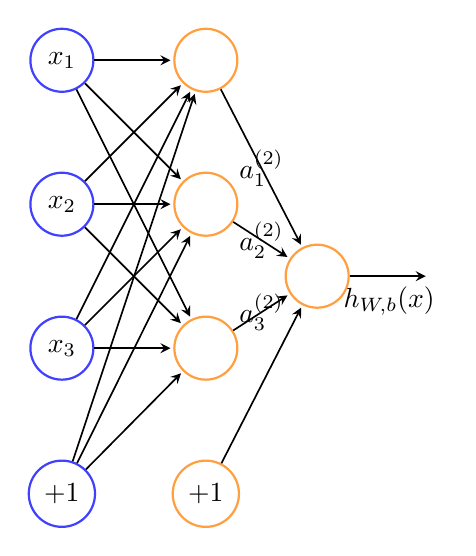
\begin{tikzpicture}
    \node[inputnode] (x1) {$x_1$};
    \node[inputnode, below=of x1] (x2) {$x_2$};
    \node[inputnode, below=of x2] (x3) {$x_3$};
    \node[inputnode, below=of x3] (b1) {$+1$};
    
    \node[hiddennode, right=of x1] (h1) {};
    \node[hiddennode, below=of h1] (h2) {};
    \node[hiddennode, below=of h2] (h3) {};
    \node[hiddennode, below=of h3] (b2) {$+1$};
    
    \node[outputnode, right=of h1, between=h2 and h3] (o1) {};
    \node[right=of o1] (o) {};
    
    \path[edgepath]
        (x1) edge node {} (h1)
        (x1) edge node {} (h2)
        (x1) edge node {} (h3)
        (x2) edge node {} (h1)
        (x2) edge node {} (h2)
        (x2) edge node {} (h3)
        (x3) edge node {} (h1)
        (x3) edge node {} (h2)
        (x3) edge node {} (h3)
        (b1) edge node {} (h1)
        (b1) edge node {} (h2)
        (b1) edge node {} (h3)
        (h1) edge node {$a_1^{(2)}$} (o1)
        (h2) edge node {$a_2^{(2)}$} (o1)
        (h3) edge node {$a_3^{(2)}$} (o1)
        (b2) edge node {} (o1)
        (o1) edge node[below] {$h_{W,b}(x)$} (o);
    \end{tikzpicture}
    
    This neural network represents the following computation:
    \begin{align*}
        a_1^{(2)} &= 
        \phi\left(W_{11}^{(1)}x_1+W_{12}^{(1)}x_2+W_{13}^{(1)}x_3+b_1^{(1)}\right)\\
        a_2^{(2)} &= 
        \phi\left(W_{21}^{(1)}x_1+W_{22}^{(1)}x_2+W_{23}^{(1)}x_3+b_2^{(1)}\right)\\
        a_3^{(2)} &= 
        \phi\left(W_{31}^{(1)}x_1+W_{32}^{(1)}x_2+W_{33}^{(1)}x_3+b_3^{(1)}\right)\\
        h_{W,b}(x) &= 
        a_1^{(3)}=\phi\left(W_{11}^{(2)}a_1^{(2)}+W_{12}^{(2)}a_2^{(2)}+W_{13}^{(2)}a_3^{(2)}\right)
    \end{align*}
    
    If we extend the activation function, to work on vectors such that 
    $f([z_1,z_2,z_3])=\left[f(z_1), f(z_2), f(z_3)\right]$ then we can write 
    the previous equation in a more compact fashion:
    \begin{align*}
        z^{(2)}&=W^{(1)}x+b^{(1)}\\
        a^{(2)}&=\phi\left(z^{(2)}\right)\\
        z^{(3)}&=W^{(2)}a^{(2)}+b^{(2)}\\
        h_{W,b}(x)&=a^{(3)}=\phi\left(z^{(3)}\right)
    \end{align*}
    Which can be generalized to:
    \begin{align*}
        z^{(l+1)}&=W^{(l)}a^{(l)}+b^{(l)}\\
        a^{(l+1)}&=\phi\left(z^{(l+1)}\right)
    \end{align*}
    
    The most common neural networks, are $n_l$-layered networks where $L_1$ is 
    the input, $L_{n_l}$ the output and $L_i$ is densely connected to 
    $L_{i+1}$. In order to compute the output, we would simply have to compute 
    the activation of $L_2$, $L_3$ etc. up to layer $L_{n_l}$, this is an 
    example of a \textbf{feedforward} neural network, as there are no loops or 
    cycles.
    
    \subsection{Backpropagation}
    Suppose we have a training set $D = \{(x_1,y_1),\dots,(x_m,y_m)\}$, we can 
    then train our neural network with batch gradient descent, with the cost 
    function for single sample as:
    \begin{equation*}
        J(W,b;x,y)=\frac{1}{2}\|h_{W,b}(x)-y\|^2
    \end{equation*} 
    This is simply a (one-half) squared-error cost function. The overall cost 
    function is then defined to be:
    \begin{equation*}
        J(W,b) = 
        \frac{1}{|D|}\sum_{i=1}^{|D|}\left(\frac{1}{2}\|h_{W,b}(x_i)-y_i\|^2\right)
    \end{equation*}
    If we add a weight decay term for regularization, then it becomes:
    \begin{equation*}
        J(W,b)=\frac{1}{|D|}\sum_{i=1}^{|D|}\left(\frac{1}{2}\|h_{W,b}(x_i)-y_i\|^2\right)
        + \frac{\lambda}{2} 
        \sum_{l=1}^{n_l-1}\sum_{i=1}^{s_l}\sum_{j=1}^{s_{l+1}}\left(W_{ji}^{(l)}\right)^2
    \end{equation*}
    Our goal now, is to minimize $J(W,b)$. To train our neural network, we will 
    initialize each parameter $W_{ij}^{(l)}$ and each $b_i^{(l)}$ to a small 
    random value near zero. If they are all the same value (e.g. $0$) then they 
    will end up learning the same function such that 
    $a_1^{(2)}=a_2^{(2)}=a_3^{(2)}=\dots$ for any input $x$.
    
    Each iteration of gradient descent then updates the parameters $W,b$ as 
    follows:
    \begin{align*}
        W_{ij}^{(l)}&=W_{ij}^{(l)}-\eta \frac{\partial}{\partial 
        W_{ij}^{(l)}}J(W,b)\\
        b_i^{(l)}&=-\eta \frac{\partial}{\partial b_i^{(l)}}J(W,b)
    \end{align*}
    
    Seems simple right? But how do we do this efficiently? The backpropagation 
    algorithm is the key. The intuition is that given some training example 
    $(x,y)$, we want to do a ``forward pass'' which computes all the 
    activations throughout the network, including the output value. Then for 
    each node $i$ in layer $l$, we compute an ``error term'' $\delta_i^{(l)}$ 
    which measures how much that node was ``responsible'' for any errors in the 
    output.
    
    For $\delta_i^{(nl)}$ we can simply compute the difference between the 
    activation and the true target label $y$. For hidden units, we don't have 
    the ``correct answer'' so instead we compute $\delta_i^{(l)}$ based on 
    weighted average of the error terms of the nodes that uses $a_i^{(l)}$ as 
    input. So in detail:
    
    \begin{enumerate}
        \item Perform a feedforward pass, computing the activations for layers 
        $L_2,L_3,\dots,L_{n_l}$
        \item For each output unit $i$ in layer $n_l$, set
        \begin{align*}
            \delta_i^{(n_l)} &= \frac{\partial}{\partial z_i^{(n_l)}} 
            \frac{1}{2}\|y-h_{W,b}(x)\|^2 = \frac{\partial}{\partial 
            z_i^{(n_l)}} \frac{1}{2}
            \left(\sqrt{(y_1-z_1^{(n_l)})^2+\dots+
                (y_i-z_i^{(n_l)})^2+\dots+
                (y_{s_l}-z_{s_l}^{(n_l)})^2}\right)^2\\
            \delta_i^{(n_l)} &= -(y_i - a_i^{(n_l)}) \cdot 
            \phi'(z_i^{(n_l)})\\
        \end{align*}
        \item For $l=n_l-1, n_l-2,\dots, 2$
            For each node $i$ in $L_l$ set
            \begin{equation*}
                \delta_i^{(l)}=\left(\sum_{j=1}^{s_{l+1}}W_{ji}^{(l)}\delta_j^{(l+1)}\phi'(z_i^{(l)})\right)
            \end{equation*}
        \item We can now compute the desired partial derivatives, as:
        \begin{align*}
            \frac{\partial}{\partial W_{ij}^{(l)}}J(W,b;x,y) &= 
            a_j^{(l)}\delta_i^{(l)}\\
            \frac{\partial}{\partial b_i^{(l)}}J(W,b;x,y) &= \delta_i^{(l+1)}
        \end{align*}
    \end{enumerate}
    We can then compute the derivatives with respect to the whole data-set, for 
    the overall cost function, as:
    \begin{align*}
        \frac{\partial}{\partial W_{ij}^{(l)}} J(W,b) &= 
        \left[\frac{1}{|D|}\sum_{i=1}^{|D|}\frac{\partial}{\partial 
        W_{ij}^{(l)}} J(W,b;x_i,y_i)\right] + \lambda W_{ij}^{(l)}\\
        \frac{\partial}{\partial b_i^{(l)}} J(W,b) &= 
        \frac{1}{|D|}\sum_{i=1}^{|D|} \frac{\partial}{\partial b_i^{(l)}} 
        J(W,b;x_i, y_i)
    \end{align*}
    
    Numerical differentiation takes one evaluation of the neural net per weight 
    (\bigO{(\#weights)^2}), now with back propagation, we simply use each edge 
    in each pass \bigO{\#weights}.
    
    \subsection{Deep Nets}
    Deep nets are when we have many layers of neurons. Each layer transforms 
    the input into a ``better'' representation, and we will just repeat this 
    procedure, and keep getting ``better'' representations. Historically, this 
    has seemed to failed, this could either be because of a bad hypothesis or 
    an issue with the learning algorithm.
    
    One of the approaches to fixing this is better architecture, for example 
    the convolutional network. Others are much more data, or computing power or 
    do find better weights before we do backpropagation or maybe the field just 
    needs to mature.
    
    \subsubsection{Convolutional networks}
    These are useful for, for example image recognition. The building blocks of 
    a convolutional network are as follow:
    \begin{enumerate}
        \item Convolution
        \item Non Linearity
        \item Pooling
        \item Classification (fully connected layer)
    \end{enumerate}
    
    \subsubsection{Convolution}
    First of all, convolution is like sliding a window over the image and 
    applying some filter to it. For example we could have a simple ``filter'', 
    ``kernel'' or ``feature detector'' which is simply a $m\times n$ matrix 
    which slides over the image. For example the matrix:
    \begin{equation*}
        \begin{pmatrix}
        1 & 0\\
        0 & 1
        \end{pmatrix}
    \end{equation*}
    might slide over the input:
    \begin{equation*}
        \begin{pmatrix}
        1 & 0 & 1\\
        0 & 2 & 0\\
        1 & 0 & 3
        \end{pmatrix}
    \end{equation*}
    Since the feature detector is $2\times 2$, it will look at first top-left 4 
    numbers, then it will slide $1$ pixel right and look at the top-right 
    numbers, then the bottom-left and then the bottom right. Producing the 
    following ``feature map'':
    \begin{equation*}
        \begin{pmatrix}
        1*1 + 0*0 + 0*0 + 1*2 & 1*0 + 0*1 + 0*2 + 1*0\\
        1*0 + 0*2 + 0*1 + 1*0 & 1*2 + 0*1 + 0*1 + 1*3 
        \end{pmatrix} = \begin{pmatrix}
        3 & 0\\
        0 & 5
        \end{pmatrix}
    \end{equation*}
    The size of the ``feature map'' is controlled by three parameers:
    \begin{itemize}
        \item Depth corresponding to the number of filters
        \item Stride is the number of pixels or indices we move the feature 
        detector with. In the above example it was 1
        \item Zero-padding, we might zero-pad in order to be able to slide the 
        window around the  edges of the matrix as well. Zero-padded convolution 
        is also called \textit{wide convolution} while non-zero-padded is 
        called \textit{narrow convolution}
    \end{itemize}
    
    \subsubsection{Non-linearity}
    The non-linearity operation aims to introduce some non-linearity into the 
    data, as it real world data is often non-linear. An example of such an 
    operation is the ReLU opeartion, which simply sets any negative elements to 
    $0$. The result is the Rectified Feature Map
    
    \subsubsection{Pooling}
    Pooling reduces the dimensionality of each feature map but retains the most 
    important information. Pooling can be done in a number of different way 
    like Max, Average, Sum etc. It runs a window over the rectified feature 
    map, and runs some function on the entries in the window. It might, for 
    example, output the maximum value in the window, resulting in a smaller 
    feature map.
    
    \subsubsection{Fully connected layer}
    The result of one or more convolution and poolings, can then be put through 
    the fully connected layer which will try to use the information to perform 
    e.g. classification, as usual.
    
    \subsection{PCA}
    PCA tries to take some data in dimension $d$ in to some dimension $k$. A 
    neural net autoencoder can come up with something very similar to this.
    
    \subsection{Autoencoder}
    
    This is an auto-encoder:
    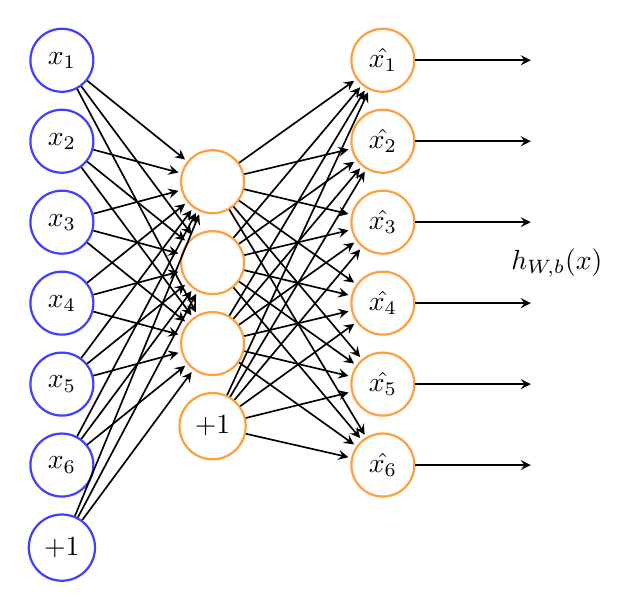
\begin{tikzpicture}[node distance = 0.2cm and 1.5cm]
    \node[inputnode] (x1) {$x_1$};
    \node[inputnode, below=of x1] (x2) {$x_2$};
    \node[inputnode, below=of x2] (x3) {$x_3$};
    \node[inputnode, below=of x3] (x4) {$x_4$};
    \node[inputnode, below=of x4] (x5) {$x_5$};
    \node[inputnode, below=of x5] (x6) {$x_6$};
    \node[inputnode, below=of x6] (b1) {$+1$};
    
    \node[hiddennode, right=of x1, between=x2 and x3] (h1) {};
    \node[hiddennode, below=of h1] (h2) {};
    \node[hiddennode, below=of h2] (h3) {};
    \node[hiddennode, below=of h3] (b2) {$+1$};
    
    \node[right=of x1] (xx1) {};
    
    \node[outputnode, right=of xx1] (o1) {$\hat{x_1}$};
    \node[right=of o1] (oo1) {};
    
    \node[outputnode, below=of o1] (o2) {$\hat{x_2}$};
    \node[right=of o2] (oo2) {};
    
    \node[outputnode, below=of o2] (o3) {$\hat{x_3}$};
    \node[right=of o3] (oo3) {};
    
    \node[outputnode, below=of o3] (o4) {$\hat{x_4}$};
    \node[right=of o4] (oo4) {};
    
    \node[outputnode, below=of o4] (o5) {$\hat{x_5}$};
    \node[right=of o5] (oo5) {};
    
    \node[outputnode, below=of o5] (o6) {$\hat{x_6}$};
    \node[right=of o6] (oo6) {};
    
    \node[textbox, right=of oo1, between=o3 and o4] (t) {$h_{W,b}(x)$};
    
    \path[edgepath]
    (x1) edge node {} (h1)
    (x1) edge node {} (h2)
    (x1) edge node {} (h3)
    (x2) edge node {} (h1)
    (x2) edge node {} (h2)
    (x2) edge node {} (h3)
    (x3) edge node {} (h1)
    (x3) edge node {} (h2)
    (x3) edge node {} (h3)
    (x4) edge node {} (h1)
    (x4) edge node {} (h2)
    (x4) edge node {} (h3)
    (x5) edge node {} (h1)
    (x5) edge node {} (h2)
    (x5) edge node {} (h3)
    (x6) edge node {} (h1)
    (x6) edge node {} (h2)
    (x6) edge node {} (h3)
    (b1) edge node {} (h1)
    (b1) edge node {} (h2)
    (b1) edge node {} (h3)
    (h1) edge node {} (o1)
    (h2) edge node {} (o1)
    (h3) edge node {} (o1)
    (h1) edge node {} (o2)
    (h2) edge node {} (o2)
    (h3) edge node {} (o2)
    (h1) edge node {} (o3)
    (h2) edge node {} (o3)
    (h3) edge node {} (o3)
    (h1) edge node {} (o4)
    (h2) edge node {} (o4)
    (h3) edge node {} (o4)
    (h1) edge node {} (o5)
    (h2) edge node {} (o5)
    (h3) edge node {} (o5)
    (h1) edge node {} (o6)
    (h2) edge node {} (o6)
    (h3) edge node {} (o6)
    (b2) edge node {} (o1)
    (b2) edge node {} (o2)
    (b2) edge node {} (o3)
    (b2) edge node {} (o4)
    (b2) edge node {} (o5)
    (b2) edge node {} (o6)
    (o1) edge node {} (oo1)
    (o2) edge node {} (oo2)
    (o3) edge node {} (oo3)
    (o4) edge node {} (oo4)
    (o5) edge node {} (oo5)
    (o6) edge node {} (oo6);
    \end{tikzpicture}
    The autoencoder tries to learn a function $h_{W,b}\approx x$, i.e. it takes 
    the input and tries to re-create it. This can be useful, as it effectively 
    tries to learn what features in the data is important if I have to know the 
    difference between two inputs but I can only do it in e.g. half the space. 
    So if there some of the input features are correlated, then this algorithm 
    will be able to discover some of those correlations. In fact it often ends 
    up learning a low-dimensional representation very similar to PCA's.
    
    \subsection{Regularization}
    We introduced weight decay regularization already, another good way to 
    regularize neural networks is the simple ``dropout'' technique, which 
    simply means that we ignore the output of some random neurons. This forces 
    the hidden neurons to be robust and approcimates averaging of exponentially 
    many models.
    
    \subsection{Finding a good local minimum}
    Our neural network is riddled with local minimum, so in order to find a 
    good local minimum, we will simply start the gradient descent from many 
    different starting points, so we end up in different local minimums and 
    choose the best one, hoping that it is a global minimum.
\end{document}